\section{The Octo Model}
\label{sec:approach}
In this section, we describe the \method{} model, our open-source generalist robot policy that can be adapted to new robots and tasks --- including new sensory inputs and action spaces --- via finetuning. We discuss the key design decisions, training objectives, training dataset, and infrastructure.
The design of the \method{} model emphasizes flexibility and scale: it supports a variety of commonly used robots, sensor configurations, and actions while providing a generic and scalable recipe that can be trained on large amounts of data.
It also supports natural language instructions, goal images, observation histories, and multi-modal, chunked action prediction via diffusion decoding~\citep{chi2023diffusionpolicy}. Furthermore, we designed \method{} specifically to enable efficient finetuning to new robot setups, including robots with different action spaces and different combinations of cameras and proprioceptive information. This design was selected to make \method{} a flexible and broadly applicable generalist robot policy that can be utilized for a variety of downstream robotics applications and research projects.


\subsection{Architecture}
\label{sec:arch}

At its core, \method{} is a transformer-based policy $\pi$. It consists of three key parts: \textbf{input tokenizers} that transform language instructions $\ell$, goals $g$, and observation sequences $o_1, \dots, o_H$ into tokens $\big[\mathcal{T}_l, \mathcal{T}_g, \mathcal{T}_o\big]$ (\cref{fig:architecture}, left); a \textbf{transformer backbone} that processes the tokens and produces embeddings $e_l, e_g, e_o = T(\mathcal{T}_l, \mathcal{T}_g, \mathcal{T}_o)$ (\cref{fig:architecture}, top); and \textbf{readout heads} $R(e)$ that produce the desired outputs, \ie actions $a$.

\paragraph{Task and observation tokenizers} We convert task definitions (\eg language instructions $\ell$ and goal images $g$) and observations $o$ (\eg wrist and third-person camera streams) into a common ``tokenized'' format using modality-specific tokenizers (see~\cref{fig:architecture}, left): 
\begin{itemize}
    \item \textbf{Language inputs} are tokenized, then passed through a pretrained transformer that produces a sequence of language embedding tokens. We use the \texttt{t5-base} (111M) model \citep{2020t5}.
    \item \textbf{Image observations and goals} are passed through a shallow convolution stack, then split into a sequence of flattened patches~\citep{dosovitskiy2020image}.
\end{itemize}

We assemble the input sequence of the transformer by adding learnable position embeddings $p$ to task and observation tokens and then arranging them sequentially $\big[\mathcal{T}_T, \mathcal{T}_{o,1}, \mathcal{T}_{o,2}, \dots\big]$.

\paragraph{Transformer backbone and readout heads} Once the inputs have been cast to a unified token sequence, they are processed by a transformer (see~\cref{fig:architecture}, top). This is similar to prior works that train transformer-based policies on sequences of observations and actions~\citep{wu2023masked,radosavovic2023robot}. The attention pattern of the \method{} transformer is block-wise masked: observation tokens can only attend causally to tokens from the same or earlier time steps $\mathcal{T}_{o, 0:t}$ as well as task tokens $\mathcal{T}_T$ (green). Tokens corresponding to non-existing observations are fully masked out (\eg a dataset without language instructions). This modular design enables us to add and remove observations or tasks during finetuning (see below). In addition to these input token blocks, we insert learned \emph{readout tokens} $\mathcal{T}_{R,t}$ (purple). A readout token at $\mathcal{T}_{R,t}$ attends to observation and task tokens before it in the sequence, but is not attended to by \textit{any} observation or task token --- hence, they can only passively read and process internal embeddings without influencing them. Readout tokens act similarly to the \texttt{[CLS]} token in BERT, serving as a compact vector embedding of the observation sequence thus far. A lightweight ``action head'' that implements the diffusion process is applied to the embeddings for the readout tokens. This action head predicts a ``chunk" of several consecutive actions, similar to prior work \cite{zhao2023learning, chi2023diffusionpolicy}. 

Our design allows us to flexibly add new task and observation inputs or action output heads to the model during downstream finetuning. When adding new tasks, observations, or loss functions downstream, we can wholly retain the pretrained weights for the transformer, only adding new positional embeddings, a new lightweight encoder, or the parameters of the new head as necessitated by the change in specification (see~\cref{fig:architecture}, bottom). This is in contrast to prior architectures \citep{brohan2022rt, shah2023vint}, where adding or removing an image input or changing the task specification would require re-initializing or re-training large components of the pre-trained model.

This flexibility is crucial to make \method{} a truly ``generalist'' model: since we cannot cover all possible robot sensor and action configurations during pretraining, being able to adapt \method's inputs and outputs during finetuning makes it a versatile tool for the robotics community. Prior model designs that use standard transformer backbones or fuse visual encoders with MLP output heads lock in the type and order of inputs expected by the model. In contrast, switching the observation or task for \method{} \emph{does not} require re-initializing most of the model.


\subsection{Training data}
\label{sec:train_data}

\begin{figure}[t]
\vspace{-0.3cm}
   \centering
   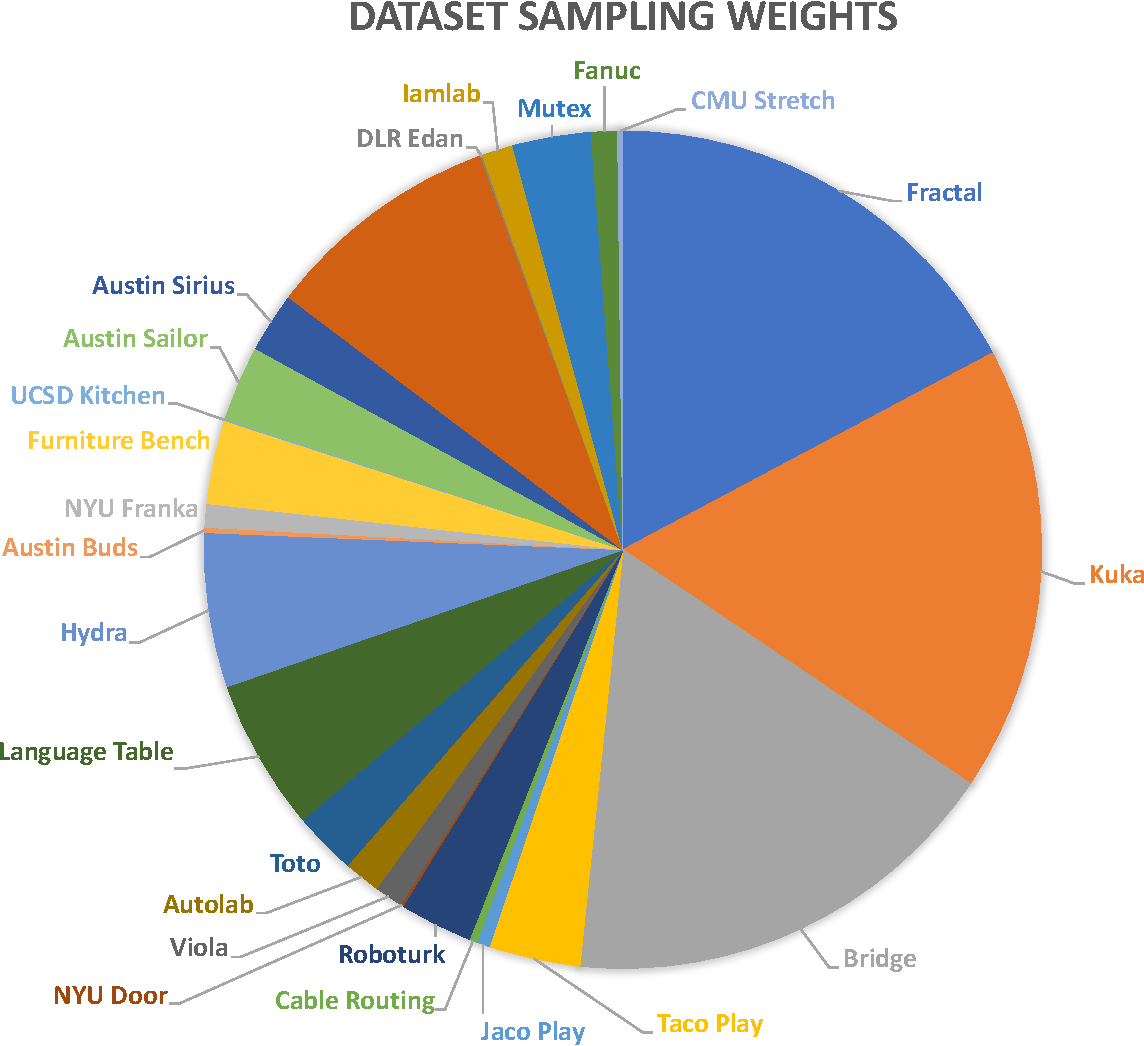
\includegraphics[width=\linewidth]{figures/sampling_weights.pdf}
   \caption{\textbf{Training dataset composition.}
    We curate a subset of \ndatasets{}~datasets from the Open X-Embodiment dataset that have image observations, end-effector actions, and show diverse behaviors. The pie chart visualizes the fractions that each dataset contributes to every training batch on average. The dataset weights are determined by the number of samples in each dataset with small modifications to balance dataset size and diversity (see \cref{sec:train_data} for details).}
    \label{fig:datamix}
\end{figure}
We train \method{} on a mixture of \ndatasets{} datasets from the Open X-Embodiment Dataset~\citep{open_x_embodiment_rt_x_2023}, a diverse collection of robot learning datasets. Our training mixture includes demonstration data of a variety of tasks from several robot embodiments and scenes. These datasets are heterogeneous not just in terms of the robot type, but also in the sensors (e.g., including or not including wrist cameras) and labels (e.g., including or not including language instructions). See~\cref{fig:datamix} and Appendix~\ref{sec:app:data_mix} for the detailed mixture. 
To create our training mixture $D$, we curate the data by first removing all Open-X datasets that contain no image streams, as well as those that do not use
delta end-effector control. We 
also remove datasets that are too repetitive, have a low image resolution, or consist of excessively niche tasks. For the remaining datasets, we roughly categorize them into ``more diverse'' and ``less diverse'' datasets based on the tasks and environments, and then double the weight of the more diverse datasets during training.
We also down-weight a few datasets with many repetitive episodes to avoid dominating the mixture. Finally, we zero-pad any missing camera channels and align the gripper action spaces between the datasets such that a gripper command of +1 means ``the gripper is open'' and 0 means ``the gripper is closed.'' While we found the resulting training mixture to work well, future work should perform a more thorough analysis of data mixture quality for pretraining general robot policies.

\begin{figure*}[t]
    \centering
    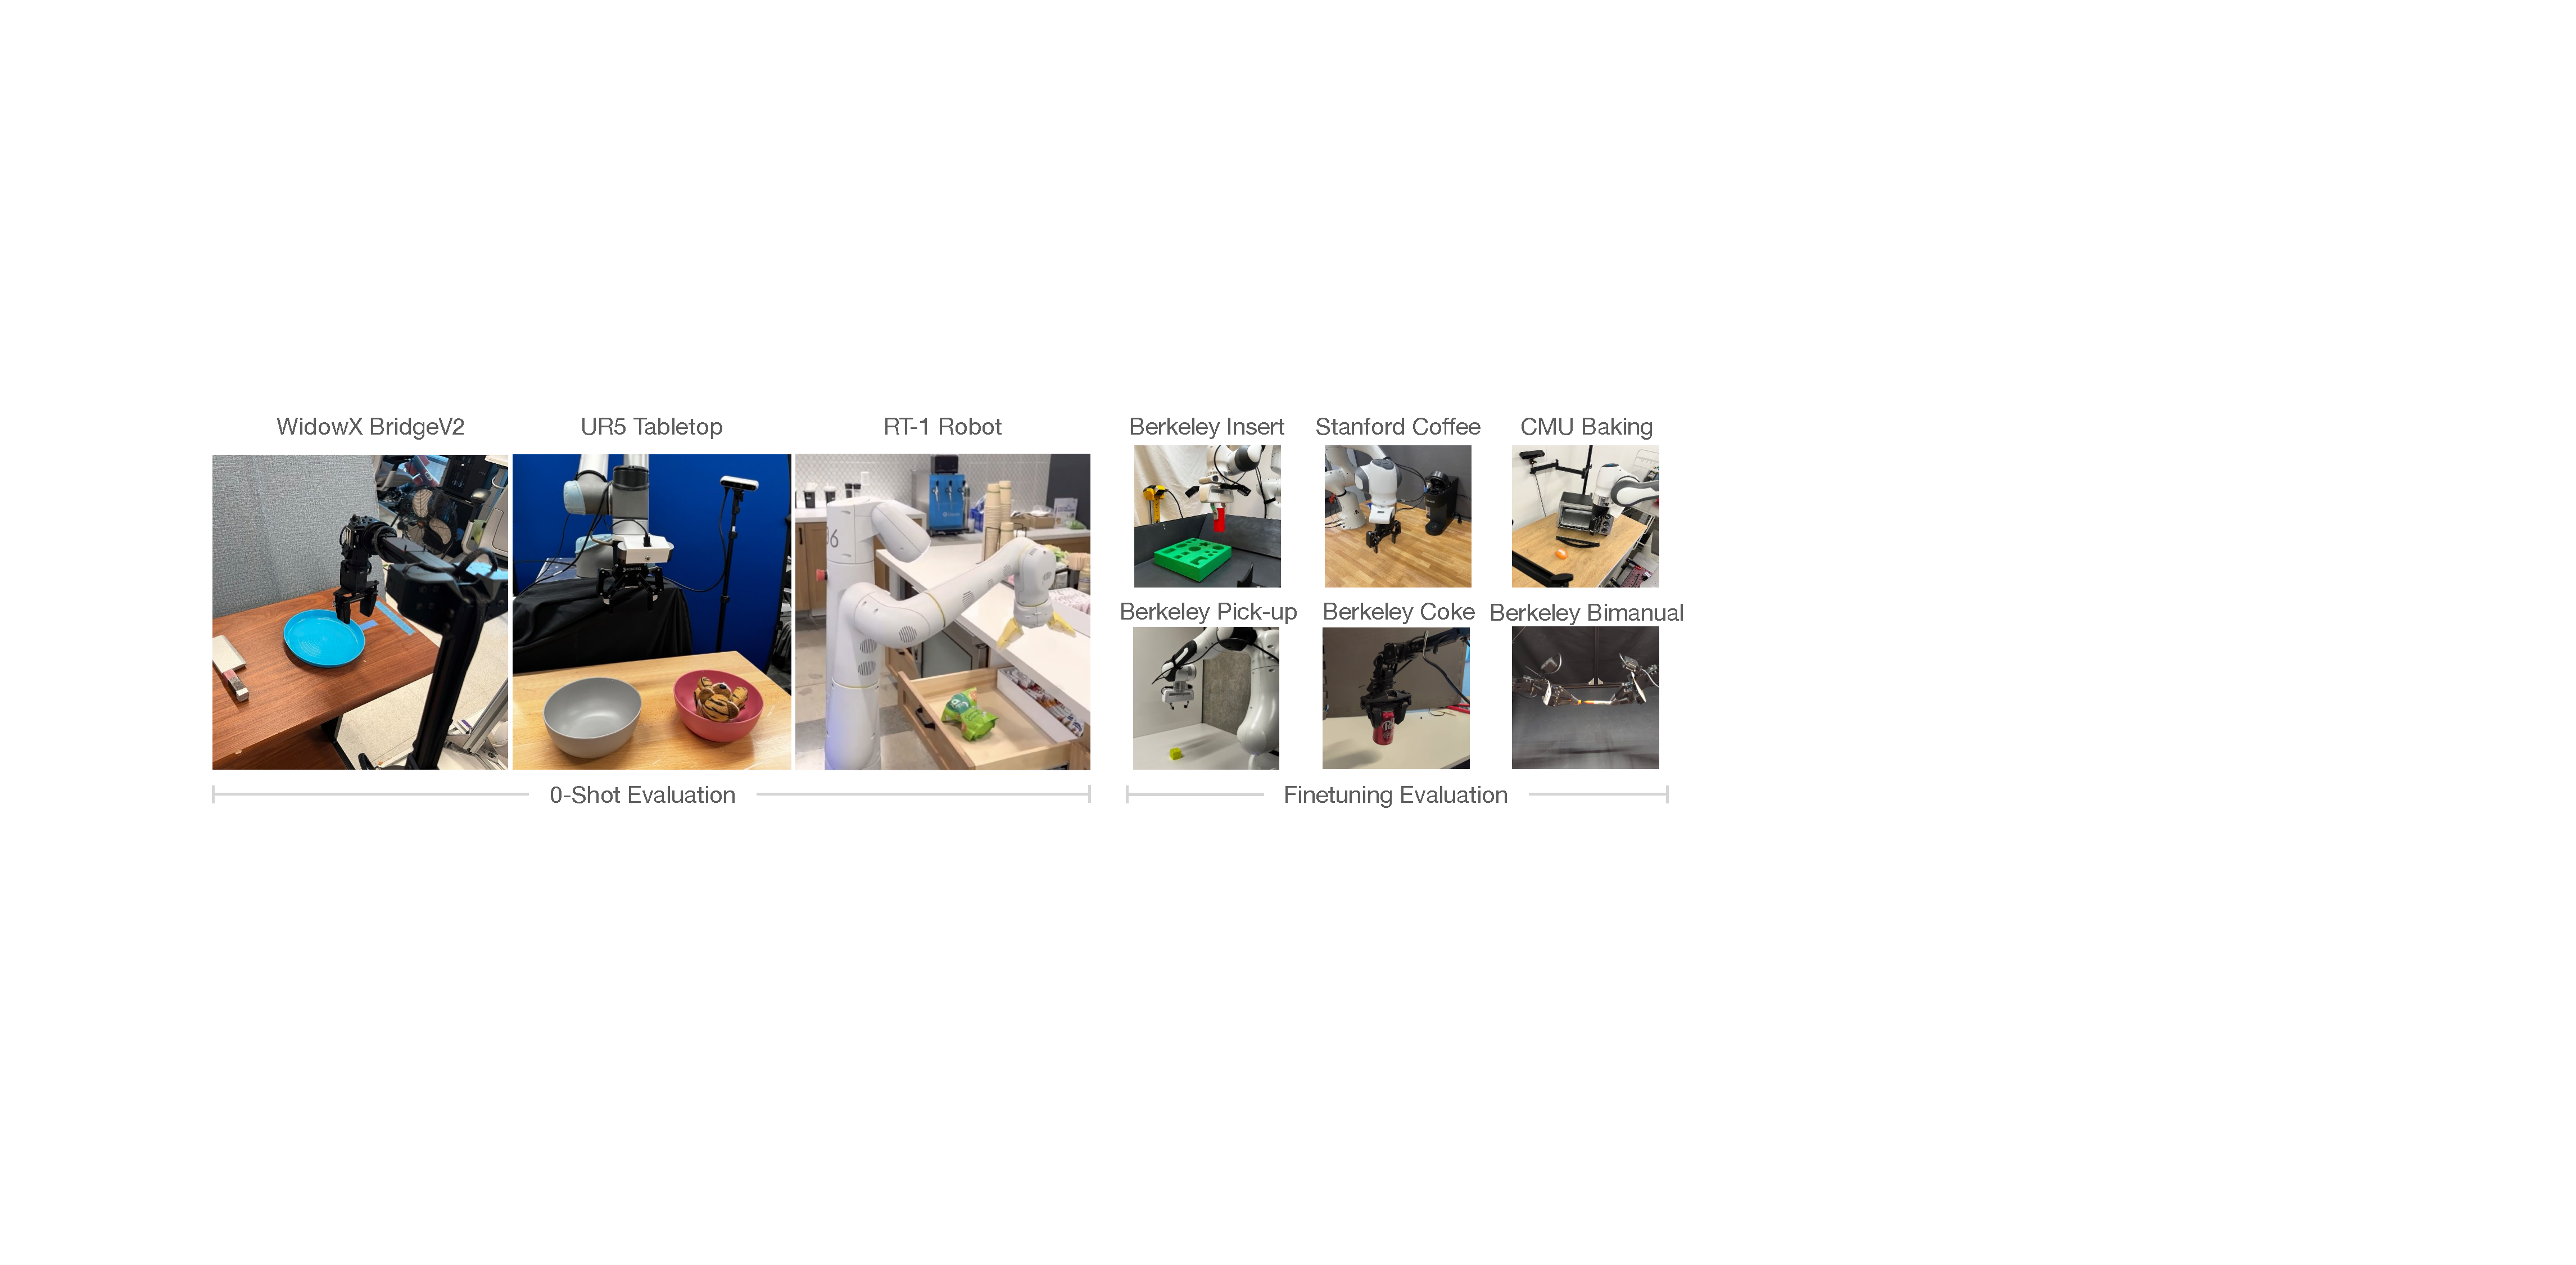
\includegraphics[width=\textwidth]{figures/eval_setups.pdf}
    \caption{\textbf{Evaluation Tasks.} We evaluate \method{} on \nsetups{}~real robot setups across \ninstitutions{}~institutions. Our evaluations capture diverse object interactions (\eg ``WidowX BridgeV2''), long task horizons (\eg ``Stanford Coffee'') and precise manipulation (\eg ``Berkeley Peg Insertion''). We evaluate \method{}'s capabilities to control robots in environments from the pretraining data out-of-the-box and to efficiently finetune to new tasks and environments with small target domain datasets. We also test finetuning with new observations (force-torque inputs for ``Berkeley Peg Insertion''), action spaces (joint position control in ``Berkeley Pick-Up'' and ``Berkeley Bimanual'') and new robot embodiments (\eg ``Berkeley Bimanual'' and ``Berkeley Coke'').}
    \label{fig:eval_setups}
\end{figure*}

\subsection{Training objective}
\label{sec:train_objective}

We use a conditional diffusion decoding head to predict continuous, multi-modal action distributions~\citep{ho2020denoising,chi2023diffusionpolicy}. Importantly, only one forward pass of the transformer backbone is performed per action prediction, after which the multi-step denoising process is carried out entirely within the small diffusion head. We found this policy parameterization to outperform policies trained with MSE action heads or discretized action distributions~\citep{brohan2022rt} in both zero-shot and finetuning evaluations. To generate an action, we sample a Gaussian noise vector $x^K \sim \mathcal{N}\big(0, I\big)$ and apply $K$ steps of denoising with a learned denoising network $\epsilon_\theta(x^k, e, k)$ that is conditioned on the output $x^k$ of the previous denoising step, the step index $k$, and the output embedding $e$ of the transformer action readout: 
\begin{equation}
    x^{k-1} = \alpha (x^k - \gamma \epsilon_\theta(x^k, e, k) + \mathcal{N}\big(0, \sigma^2I\big)).
\end{equation}
The hyperparameters $\alpha$, $\gamma$, and $\sigma$ correspond to the noise schedule: we use the standard cosine schedule from~\cite{nichol2021improved}.
We train the diffusion head using the standard DDPM objective first proposed in \cite{ho2020denoising}, where we add Gaussian noise to the dataset actions and train the denoising network $\epsilon_\theta(x^k, e, k)$ to reconstruct the original action.
For a detailed explanation of diffusion policy training, see \citet{chi2023diffusionpolicy}. We list all hyperparameters in Appendix~\ref{sec:app:hyperparams}.

We use the same diffusion training objective during finetuning and update the full model, a recipe which outperformed those that freeze subsets of the pretrained parameters. In all finetuning experiments, we employ the same recipe: given a small target domain dataset with around 100 trajectories, we finetune for 50k steps using a cosine decay learning rate decay with linear warmup.


\subsection{Training Details}
\label{sec:training_details}
We trained two variants of our model: \method-Small with a transformer backbone that mirrors the size of a ViT-S, and \method-Base with a transformer backbone that mirrors the size of a ViT-B~\citep{dosovitskiy2020image}. 

We use the AdamW optimizer~\citep{loshchilov2017decoupled} with an inverse square root decay learning rate schedule~\citep{zhai2022scaling}, with weight decay of 0.1 and gradient clipping of 1.0. The ViT-B was trained for 300k~steps with a batch size of $2048$ using a TPU v4-128 pod, which took 14~hours. A finetuning run of the same model on a single NVIDIA~A5000 GPU with 24GB of VRAM takes approximately 5~hours and can be sped up with multi-GPU training. 

We train using 2 frames of observation history; in our preliminary experiments, we found significantly diminishing gains beyond the first additional frame. We use hindsight goal relabeling~\citep{andrychowicz2017hindsight}, which selects a state uniformly from the future in the trajectory to assign as the goal image, similar to prior work \citep{lynch2020language, walke2023bridgedata, shah2023vint,rosetebeas2022latent,mees2023grounding}. We apply common image data augmentations during training, and randomly zero out the language instruction or goal image per training example to enable \method{} to be conditioned on \emph{either} language instructions \emph{or} goal images. For datasets without language annotations, we always use goal image conditioning. This enables our model to learn control mostly from self-supervised visual observations and reduces the burden on language annotation, similar to prior work on multi-context imitation learning~\citep{lynch2020language,mees2022calvin,mees2022matters,mees2023grounding}. For more details on the choice of hyperparameters, see Appendix~\ref{sec:app:hyperparams}.


\subsection{Model Checkpoints \& Code}
\label{sec:code}

We open-source all resources required to train, finetune and run our model (see \website):
\begin{itemize}
    \item \textbf{Pretrained \method{} checkpoints} for \method-Small (\smallnparams{}~params) and \method-Base (\largenparams{}~params). %
    \item \textbf{Finetuning scripts} for \method{} models, in JAX.
    \item \textbf{Model pretraining pipeline} for \method{} pretraining on the Open X-Embodiment dataset, in JAX.
    \item \textbf{Standalone data loaders} for Open X-Embodiment data, compatible with JAX and PyTorch.
\end{itemize}
We provide a simple example for loading and running a pretrained \method{} model in Appendix~\ref{sec:app:code_example}.
